\documentclass[UFT8]{beamer}
\usepackage{tikz}
\usetikzlibrary{arrows, positioning, shapes.geometric, arrows.meta}

\mode<presentation> {
	\usetheme{Frankfurt}
	% or AnnArbor Antibes Bergen Berkeley Berlin Boadilla boxes CambridgeUS Copenhagen Darmstadt default Dresden Frankfurt Goettingen Hannover Ilmenau JuanLesPinsLuebeck Madrid Malmoe Marburg Montpellier PaloAlto Pittsburgh Rochester Singapore Szeged Warsaw
	
	\setbeamercovered{transparent}
	% or whatever (possibly just delete it)
}

\usepackage{color}
\usepackage{algorithm,algpseudocode}
\usepackage{algorithmicx}
\usepackage{algpseudocode}
\usepackage{amsmath}
\usepackage{float}

\usefonttheme[onlymath]{serif}

% \documentclass[ppt.tex]{subfiles}
\begin{document}

\section{{Soundness}}

\begin{frame}
    \frametitle{Argument of NP relation}
    \begin{itemize}
        \item Given cyclic group $\mathbb{G}$ of order $p$, $g$ is its generator. 
        \item NP relation $\mathcal{R} = (x; w)$ such that $g^w = x$.
        \item $\mathcal{L}(\mathcal{R}) = \mathbb{G}$ is in P! Proving $x\in \mathcal{L}(\mathcal{R})$ is trivial.
    \end{itemize}

    Prover argues its possession of witness of $x$.

    \quad

    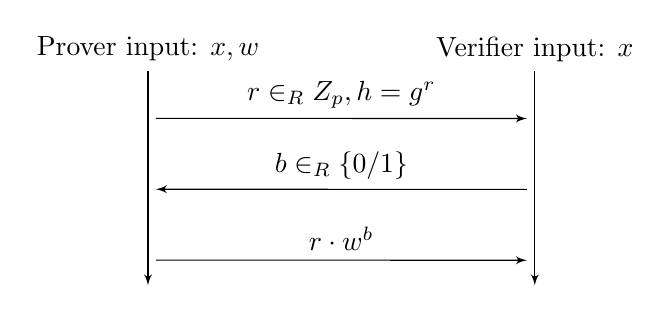
\begin{tikzpicture}[auto, node distance=2cm,>=latex']
		\node [rectangle, align=center] (prover) {Prover input: $x, w$};
		\node [rectangle, right=of prover, align=center] (verifier) {Verifier input: $x$};
	
		\draw[->] (prover) -- +(0, -30mm);
		\draw[->] (verifier) -- +(0, -30mm);
	
		\draw[->] ([yshift=-6mm, xshift=1mm]prover.south) -- node {$r \in_R \mathbb{Z}_p, h=g^r$} ([yshift=-6mm, xshift=-1mm]verifier.south);
		\draw[<-] ([yshift=-15mm, xshift=1mm]prover.south) -- node {$b \in_R \{0/1\}$} ([yshift=-15mm, xshift=-1mm]verifier.south);
        \draw[->] ([yshift=-24mm, xshift=1mm]prover.south) -- node {$r \cdot w^b$} ([yshift=-24mm, xshift=-1mm]verifier.south);
	\end{tikzpicture}

    The protocol is of exactly $1/2$-soundness.

\end{frame}

\begin{frame}
    \frametitle{Knowledge Soundness}
    \begin{definition}[knowledge soundness]
        A proof system has knowledge soundness with error $\kappa$ if there exists an extractor $K$, such that for every $\mathcal{A}$, if $P^*$ convinces $V$ of $x$ with probability $\epsilon > \kappa$, then $K^{\mathcal{A}(\cdot)}(x)$ outputs $w$ s.t. $(x, w) \in R$ in expected time
        $$
        \frac{poly(|x|)}{\epsilon(|x|) - \kappa(|x|)}
        $$
    \end{definition}

    If prover can pass the verification with probability $1/2 + \epsilon$.
    For each $h$, extractor queries $\mathcal{A}$ with both $b = 0, 1$.
    \begin{equation*}
        \Pr[h \leftarrow \mathcal{A}; \mathcal{A} \text{ can answer both } r \text{ and } rw] \ge 2\epsilon
    \end{equation*}

    Extractor can extract $w$ in expected $1 / 2\epsilon$ repetitions, though $1 / 2\epsilon$ might be super-polynomial.
\end{frame}


\begin{frame}
    \frametitle{Witness-extended Soundness}
    \begin{definition}[Witness-Extended Emulation, from Butlletproof]
        \begin{align*}
            & \Pr\left[
                \mathcal{A}_1(tr) = 1 : \begin{aligned}
                \sigma \leftarrow Setup(1^\lambda), \\
                (u, s) \leftarrow \mathcal{A}_2(pp), \\
                tr \leftarrow \langle \mathcal{P}^*(\sigma, u, s), \mathcal{V}(\sigma, u) \rangle
            \end{aligned} 
            \right] \\
            = & \Pr\left[ \begin{aligned}
                \mathcal{A}_1(tr) = 1 \land \\
                (tr \text{ is accepting} \Rightarrow \\
                (\sigma, u, w) \in \mathcal{R})
            \end{aligned}: \begin{aligned}
                \sigma \leftarrow Setup(1^\lambda), \\
                (u, s) \leftarrow \mathcal{A}_2(pp), \\
                (tr, w) \leftarrow \mathcal{E}^{\mathcal{O}}(\sigma, u)
            \end{aligned} 
            \right]
        \end{align*}
    \end{definition}
    $\mathcal{E}$ outputs
    \begin{itemize}
        \item The honest verifier's view of an execution of the proof of knowledge with the specified prover
        \item The witness for the statement being proved in the proof of knowledge
    \end{itemize}
\end{frame}

\begin{frame}
    \frametitle{Tree Transcript}
    \begin{itemize}
        \item $(2, 3)$-tree transcript
    \end{itemize}
    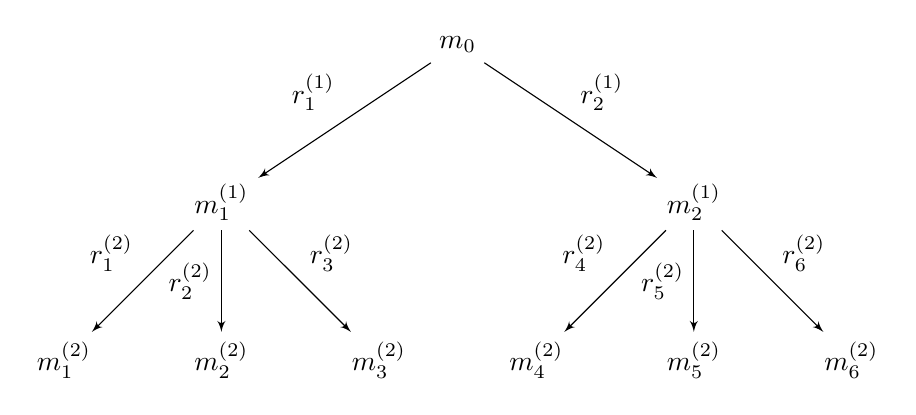
\begin{tikzpicture}[auto, node distance=2.5cm,>=latex']
		\node at (3, 0) (m_0) {$m_0$};
        \node at (0, -2) (m_1_1) {$m^{(1)}_1$};
        \node at (6, -2) (m_1_2) {$m^{(1)}_2$};
        \draw[<-] (m_1_1) -- node {$r^{(1)}_1$} (m_0);
        \draw[->] (m_0) -- node {$r^{(1)}_2$} (m_1_2);
        
        \node at (-2, -4) (m_2_1) {$m^{(2)}_1$};
        \node at (0, -4) (m_2_2) {$m^{(2)}_2$};
        \node at (2, -4) (m_2_3) {$m^{(2)}_3$};
        \draw[<-] (m_2_1) -- node {$r^{(2)}_{1}$} (m_1_1);
        \draw[<-] (m_2_2) -- node {$r^{(2)}_{2}$} (m_1_1);
        \draw[->] (m_1_1) -- node {$r^{(2)}_3$} (m_2_3);
        
        \node at (4, -4) (m_2_4) {$m^{(2)}_4$};
        \node at (6, -4) (m_2_5) {$m^{(2)}_5$};
        \node at (8, -4) (m_2_6) {$m^{(2)}_6$};
        \draw[<-] (m_2_4) -- node {$r^{(2)}_{4}$} (m_1_2);
        \draw[<-] (m_2_5) -- node {$r^{(2)}_{5}$} (m_1_2);
        \draw[->] (m_1_2) -- node {$r^{(2)}_6$} (m_2_6);
	\end{tikzpicture}
\end{frame}

\begin{frame}
    \frametitle{Special Soundness}
    \begin{definition}[Special soundness, from ProtoStar]
        Let $\mu, N \in \mathbb{N}$ and $(a_1, \cdots, a_{\mu}) \in \mathbb{N}^\mu$.
        A $(2\mu + 1)$-move public coin interactive proof $\Pi$ for relation $\mathcal{R}$ where the verifier samples its challenges from a set of size $N$ is $(a_1, \cdots, a_{\mu})$-out-of-$N$ special-sound if there exists a polynomial time algorithm that, on input $x$ and any $(a_1, \cdots, a_{\mu})$-tree transcript for $\Pi$ outputs $w \in \mathcal{R}(x)$.
    \end{definition}

    Sigma protocol is 2-special sound.

    \begin{theorem}[Forking Lemma]
        Let $(P, V)$ be a public coin interative protocol has special soundness, then $(P, V)$ has witness-extended emulation.
    \end{theorem}

    Special soundess $\ge$ Witness-extended emulation $=$ Knowledge soundness
\end{frame}

\begin{frame}
    \frametitle{Round by round Soundness}
    Round by round soundness is resistant to state restoration attack:
    \begin{itemize}
        \item Given a false claim $x$, the game initializes the set of $S = \{ null \}$.
        \item Repeat the following at most $T$ times, where $T = poly(\lambda)$:
        \begin{itemize}
            \item $P^*$ chooses an element $cvs$ in $S$.
            \item The game sets $\mathcal{V}$'s state to $cvs$.
            \item If $cvs = null$: $\mathcal{P}^*$ sends $m_1$ to $\mathcal{V}$. 
            Then $\mathcal{V}$ returns a random point $r_1$ to $\mathcal{P}^*$;
            Add $m_1 || r_1$ into $S$.
            \item If $cvs = m_1 || r_1 || \cdots || m_{i-1} || r_{i-1}$: $\mathcal{P}^*$ sets $\mathcal{V}$'s state to $cvs$, generates $m_i$ and sends it to $\mathcal{V}$. 
            After receiving $r_i$ samples by $\mathcal{V}$, $\mathcal{P}^*$ adds $cvs || m_i || r_i$ into $S$.
        \end{itemize}
        \item The game outputs $1$ iff there's an accepting transcript in $S$.
    \end{itemize}
\end{frame}

\end{document}